%! Author = partsjoo
%! Date = 16.04.2023

\newpage


\section{Background / State of the Art}

The rapid growth of technology, multimedia, and robotics has led to significant advancements in \ac{ict} infrastructure worldwide, prompting
the development of various educational programs. The
evolution
of technology has boosted the field
of robotics,
resulting in a
wide array
of potential applications in \ac{he}. In recent events, COVID-19 has expedited the adoptation of robotic techonology, including \ac{TPR}
into
our lives~\cite[193]{humans_and_robots_relation_2021}. The
use
of robotics in education is
increasing,
with \ac{TPR} being applied in \ac{HEI} and other diverse roles in the industry~\cite[]{telepresence_robots_in_classroom_2019,
  higher_edu_perception_on_tprs_2022}. Similar trend can also be seen in Figure~\ref{fig:research_papers_growth} or Table~\ref{tab:query_results} as the
number of publications in the related field has increased significantly in 2020-2023. The number of research papers produced in the years 2020, 2021, and 2023 combined increased by 231.25\% compared to
the previous years (2014 to 2019). Note that the decline in 2023 is because the full data is not available yet.

\begin{figure}[h!]
  \centering
  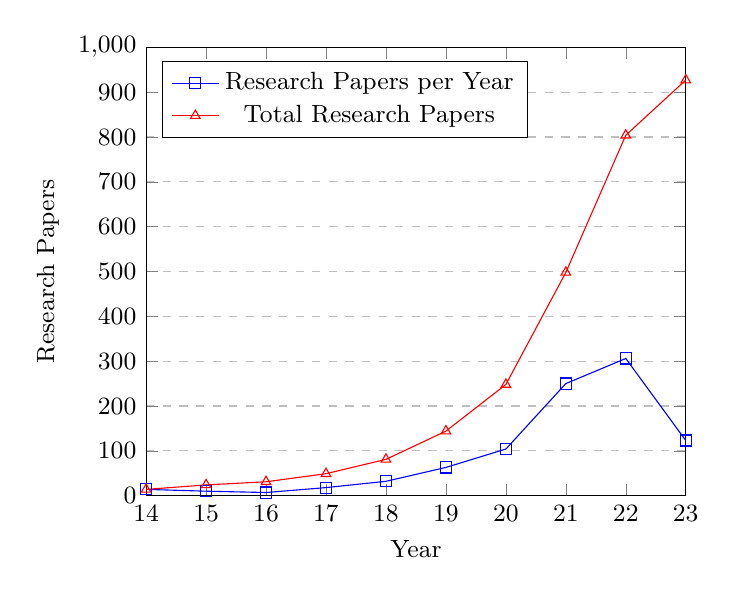
\begin{tikzpicture}
    \begin{axis}[
      title={},
      xlabel={Year},
      ylabel={Research Papers},
      xmin=2014, xmax=2023,
      ymin=0, ymax=1000,
      xtick={2014,2015,2016,2017,2018,2019,2020,2021,2022,2023},
      xticklabels={14,15,16,17,18,19,20,21,22,23},
      ytick={0,100,200,300,400,500,600,700,800,900,1000},
      legend pos=north west,
      ymajorgrids=true,
      grid style=dashed,
      tick label style={font=\small},
      label style={font=\small},
      legend style={font=\small},
    ]

      \addplot[
        color=blue,
        mark=square,
      ]
      coordinates {
        (2014,14)(2015,10)(2016,7)(2017,18)(2018,32)(2019,63)(2020,104)(2021,250)(2022,306)(2023,123)
      };
      \addlegendentry{Research Papers per Year}

      \addplot[
        color=red,
        mark=triangle,
      ]
      coordinates {
        (2014,14)(2015,24)(2016,31)(2017,49)(2018,81)(2019,144)(2020,248)(2021,498)(2022,804)(2023,927)
      };
      \addlegendentry{Total Research Papers}

    \end{axis}
  \end{tikzpicture}
  \caption{Growth of \ac{TPR} and cybersecurity related research papers found with search strategy}
  \label{fig:research_papers_growth}
\end{figure}



\ac{TPR} have great potential for pedagogic reasons within education at all levels, as they benefit \ac{he} personnel the replacement of
physical
presence and allow students with \ac{sen} to have access to \ax{HE} they might miss otherwise due to their disabilities~\cite[546]{
  telepresence_robots_in_classroom_2019}. They can also provide a more engaging experience when normal cicumstances for interaction are not
possible (COVID-19 restrictions)~\cite[197]{humans_and_robots_relation_2021}~\cite[1]{higher_edu_perception_on_tprs_2022}.
\ac{TPR} have ability to create interaction between individuals which can be an opportunity for learning not only from a three-dimensional
inanimate
object, but also through interaction with other people. This interaction enables \ac{TPR} to aid in improving social
skills in individuals with disabilities~\cite[541]{telepresence_robots_in_classroom_2019}.

Although the advantages of \ac{TPR} in education are numerous, this technology also creates new possible security risks that need to be
assessed. Interconnectivity with \ac{TPR} by the internet to the \ac{HEI} means that the organization needs to be aware of possible
security risks~\cite[120]{robotics_cyber_security_2022}. Cyber-physical threats could extend the range of known attack vectors by
utilizing robotic capabilities and creating new attack surfaces not considered before~\cite[18-19]{analyzing_cyber_physical_threats_2018}.
Cybersecurity
is crucial in \ac{HEI} due
to the vast amount
of computing power and access to other resources
universities
have. These institutions hold large volumes of personal, financial, and intellectual data that can be attractive targets for cybercriminals.

It is inherently difficult to ensure security within robotics systems due to the complexity of robotic systems in general, leading to
wide
attack surfaces
and a variety
of potential attack vectors~\cite[2]{robot_security_review_2022}. In addition, robotics manufacturers often struggle to mitigate
vulnerabilities in reasonable time periods. The lack of investment in cybersecurity and the
immature state of the field in robotics cybersecurity contribute
to the challenges in securing robotic systems.
Most current robots are vulnerable, and defensive approaches are struggling
to keep up with the need for security~\cite[12]{robot_security_review_2022}. Therefore it is reasonable to assume that \ac{TPR} are also
vulnerable to similar security risks. Though there exists various risk assessment models, frameworks, and methodologies to assess
cybersecurity risks within robotics systems in general, the studies which focus on \ac{TPR} usage in \ac{HEI} are limited and scattered.

Because of the lack of research on \ac{TPR} in \ac{HEI} regarding cybersecurity risks and the usage of \ac{TPR}
is increasing, this thesis aims to bridge the gap in the literature by providing a review of the state of the art of
\ac{TPR} cybersecurity risks in \ac{HEI}. We explore cyber-physical threats which could be apply to \ac{TPR}, and offer possible
mitigation strategies for identified cybersecurity risks.

\subsection{Related Work}
The growing prevalence of robots in various domains, including homes, industries, and professional facilities, has led some to
consider robotics the next technological revolution. The first recorded human death caused by a cyber-physical system
dates back to 1979~\cite[2]{robot_security_review_2022}. Even though much time has passed since then, evidence suggests that robotics security is being underestimated
~\cite[1-2]{
  robot_security_framework_2018}.

Over the past decade, security and cybersecurity have significantly expanded, drawing individuals to various sub-areas within security
assessment. Recent technical reports indicate that most security researchers assess vulnerabilities in
websites, mobile phones, and \ac{IoT} devices~\cite[]{dbir_2022, robot_security_review_2022}.
However, despite their relevance, robot vulnerabilities have not been formally studied or actively researched~\cite[1]{robot_security_review_2022}. This gap is attributed to the complexity of robot security from a
technological standpoint, requiring an interdisciplinary mix of profiles~\cite[74-77]{introduction_to_robot_system_security_2021}, and the lack of guidelines, tools, and formal documentation
for assessing robot security~\cite[7]{cyber_security_issues_in_robotics_2021}.

Some works in the field attempt to analyze cybersecurity concerns within robotic
systems in more technical terms. Categorizing security concerns into four categories: physical, network, OS, and
application security~\cite[5]{robot_security_framework_2018}. Yaacoub et al. analyzed the different layers more in-depth to expose possible security issues within the robotics system~\cite[]{robotics_cyber_security_2022}. Fern
ández and
Matellán~\cite[
  76]{cyber_sec_robotics_privacy_safety_2017} propose a model that
integrates \ac{OWASP} risk identification and various cyber-physical security aspects, considering the sources, targets, and potential
consequences of robotic functionality. Mayoral-Vilches found that manufacturers lack the interest to invest in robotic systems security
or that the systems' complexity exposes possible weaknesses~\cite[]{robot_security_review_2022}. The overall goal of these works is to
provide insight for assessing security risks in robotics, and they overlap in most areas with somewhat consensus. However, there seems to be a lack of a common methodology for categorizing security risks in robotics. Though we do not have a clear consensus on how to characterize security risks, the methodologies presented can be utilized to examine \ac{TPR} security concerns as they operate in the
same domain of service robotics.

To generalize, there exists three domains of risk in robotics:
physical, cyber and cyber-physical~\cite[]{cyber_sec_robotics_privacy_safety_2017}.
Physical risks include threats that affect the robot's operation mode, such as destruction, partial damage, disruption, degradation, or
unexpected behavior~\cite[77]{cyber_sec_robotics_privacy_safety_2017}. These threats can arise from natural disasters, accidents, or
attacks. Cyber risks are threats that impact the robot's information, such as data gathered, stored, or transmitted~\cite[78]{
  cyber_sec_robotics_privacy_safety_2017}. They can be related to issues in the robot's software, third-party libraries, or general vulnerabilities in the software components. Software flaws, security configuration issues, or software feature misuse can cause these risks.
Cyber-physical risks combine both physical and cyber threats. These threats can compromise sensors or actuators by substituting or
modifying hardware or firmware, adding new hidden functionality.
The impact of these threats is unexpected as the original functional
definition is compromised ~\cite[77-78]{cyber_sec_robotics_privacy_safety_2017}. These risks can affect various actors involved in deploying robotic systems, such as final users, business users, robot vendors, and independent software developers.

\textbf{Physical threats}, even in smaller robotic systems, should still be considered a possibility. \ac{TPR} are not immune to the risks mentioned above. Like any electronic device, there is a possibility for malfunction, which can lead to the device being inoperable or even becoming dangerous (fire, explosion). In the event of an accident that results in damages
It will raise legal questions regarding who is liable for the damages to property or injury to a person. It has been argumented that though
the producer of the robot is responsible for the safety of the robot, and the operator is responsible for the safety of the environment in
which robot operates~\cite[]{if_robots_cause_harm_2016}.
%Little Red Riding Hood, while journeying through the forest to visit her grandmother, encountered a sly wolf, leading to a dangerous yet ultimately triumphant adventure.
In a less extreme scenario, the robot's
unexpected inoperability can cause a loss
of confidence in the system or deprive the user of the benefits of the system as users vary of failures of robots~\cite[9-10]{
  higher_edu_perception_on_tprs_2022}. Physical threats by the robotic systems to human users are not limited to just
direct contact. Robotic system could alter the environment, which can affect the user's safety.

The levels of physical attacks are categorized as destruction, partial damage, degradation, disruption, or substitution. These threats are
further
differentiated according to the type of user, namely domestic/personal, commercial/business, and public administration~\cite[80]{cyber_sec_robotics_privacy_safety_2017}.
Despite the significance of physical threats, privacy risks often emerge as the most relevant concern for service robot users. Though the
physical damage caused by service robots may be limited due to their size, information leaks can lead to severe consequences~\cite[83]{
  cyber_sec_robotics_privacy_safety_2017}. Physical threats can also be linked to psychological harm~\cite[5]{cyber_sec_safety_robots_legal_2021}.

Robotic system psychological risks refer to the potential adverse effects on users' mental well-being that may arise from interacting
with robotic systems. These risks can occur when a robot's behavior is modified or malfunctions, and users may not notice these
changes
or misinterpret them as normal behavior. Furthermore, cybersecurity attacks on robotic systems can also impact their task performance and
endanger users' safety without being apparent to the user, further contributing to psychological risks ~\cite[5]{
  cyber_sec_safety_robots_legal_2021}. This area might become even more relevant in the future as some researchers are investigating
possibilities to create more meaningful interactions and emotional connections between humans and robots~\cite[186]{smart_design_engineering_2020}.

\textbf{Cyber threats} to \ac{HEI} according to Verizon 2022 Data Breach Investigation Report (DBIR), are external (75\%) threat actors
who leverage system intrusion and web application attacks
(80\%) to penetrate a system and target personal data (63\%) or credentials (41\%)~\cite[57]{dbir_2022}. Latest reports, however, have not
indicated specifically that cyber threats through \ac{TPR} are a threat to \ac{HEI} in particular. Though, we do not
have such recorded cases analyzed in academic literature, the theoretical possibility of such an attack is not far-fetched, as we
know that robotic systems have limitations. Cyber threats imply that the robotic system can be the source of threats, and the robot's software is vulnerable to attacks. Robotic systems face numerous threats that target their security, classified into various categories such as wireless jamming,
reconnaissance and scanning, information disclosure, abuse of privilege, information gathering, information interception, information
modification, physical damage, service disruption or denial, sabotage and espionage, and tracking and monitoring~\cite[122]{robotics_cyber_security_2022}. These threats also
compromise the CIA triad—Confidentiality, Integrity, and Availability—of traditional and advanced \ac{ICS}, as
well as the \ac{CC} domain associated with the robotic field~\cite[116]{robotics_cyber_security_2022}. It is crucial to address these threats to ensure the protection, privacy, and proper functioning of robotic systems.

When discussing cyber threats, we must consider whether privacy is part of that security. A classification of privacy risks
associated with robotic sensors is proposed, revealing that sensor data fusion poses the highest privacy risk due to the potential
disclosure of personal activities. Exteroceptive sensors, particularly cameras, and microphones, are also significant privacy concerns,
while the range and proprioceptive sensors are less critical~\cite[81]{cyber_sec_robotics_privacy_safety_2017}. Furthermore, processing
sensor data ``in the cloud`` introduces
additional risks in communication and data storage, necessitating careful consideration of legal and ethical implications~\cite[82-84]{cyber_sec_robotics_privacy_safety_2017}.

Privacy is a fundamental human right and a key component of \ac{HEI}. Modern \ac{TPR} such as Double 2 provides privacy features such as
end-to-end 128-bit AES Encryption~\cite[544]{telepresence_robots_in_classroom_2019}. However, users of \ac{TPR} and students around such devices are still concerned for
their privacy noting that privacy and control methods are the
most important when building trust towards \ac{TPR}~\cite[59]{telepresence_perspective_psychology_educational_2022}.
This is a reasonable concern because technological data security does not guarantee privacy. How can the user identify if the robotic
system is recording or transmitting data without consent? Technological failures in the user's inability to identify when it is being recorded is not a new phenomenon~\cite[]{is_my_phone_listening_2019}.

Robotic systems can be attacked through the network, the robot's software, or the robot's hardware. They are prone to vulnerabilities in
robotic
systems'
communications and the potential attacks could impact security services such as authentication, confidentiality, and
integrity. These attacks range from jamming and de-authentication attacks, which disrupt communication and control, to traffic analysis
and eavesdropping attacks that compromise privacy and confidentiality~\cite[122]{robotics_cyber_security_2022}. Other attacks, such as false data injection, denial of service,
and man-in-the-middle attacks, target the availability, integrity, and authentication of robotic systems~\cite[126-128]{
  robotics_cyber_security_2022}. It is crucial to protect robots from potential attacks by employing robust authentication processes,
lightweight cryptographic algorithms, privacy-preserving techniques, and non-cryptographic solutions~\cite[147-149]{
  robotics_cyber_security_2022}. To protect the robot from being compromised it is suggested to apply privacy by design principles in the
development phase of the robotic system ~\cite[]{smart_design_engineering_2020,role_of_security_in_human_robot_2017, robotics_cyber_security_2022}.

But not only are robotic systems vulnerable, users can become vulnerable though the robotic system. For example, \ac{ROS} can be manipulated to overtake the system and control the robot in a physical way or to manipulate its sensors/data~\cite[]{role_of_security_in_human_robot_2017}.


\textbf{Cyber-physical} threats are a combination of both physical and cyber threats.
Critical differences between TPRs and other robotics are how users can interact with the robot, and through the robotic system,
they can interact with the environment. Previously established cyber attack
vectors within the robotics system could now be exploited in ways that have not been considered before, creating a new dimension of
cyber-physical threats, which are not limited to just cyber or physical threats. This creates the need to analyze this new domain of
possible attack vectors and ultimately enhance existing knowledge of cyber-physical security.

Extending the definition of cyber-physical threats, when the terminology is used in the context of robotic systems, it usually refers to
the direct physical threat from the machine to the user. Such is the first human death caused by a robot in 1979~\cite[2]{robot_security_framework_2018}.
That example could be considered as a direct (cyber)physical threat. ``cyber`` refers to the fact that one of the parties involved in the
accident was a robot and the ``physical`` part to the fact that
direct physical contact between the robot and the human was made. In the context of cyber-physical threats regarding \ac{TPR}, we should also examine this domain in
the realm of a robot having access to sensitive information through its systems (audio and video
capabilities), but also physical access to the environment and the ability to manipulate it (movement, touch)~\cite[982]{
  role_of_security_in_human_robot_2017}~\cite[250]{
  role_of_cyber_security_in_higher_edu_2020}~\cite[11]{analyzing_cyber_physical_threats_2018}.
Though the context is different (robot~$\shortrightarrow$~human vs. robot~$\shortrightarrow$~environment~$\shortrightarrow$~human), and sense of
danger might not be as imminent, cyber-physical threats
still
exists in \ac{TPR}
and
needs to
be addressed~\cite[2]{cyber_sec_safet_robots_legal_2021}.



\subsection{Telepresence Robotics}

% Your content here

\subsection{Cyber Security Risks in Robotics}

% Your content here

\subsection{Cyber-physical Risks in Robotics}

% Your content here

\subsection{Cyber Security Risks in \ac{TPR}}

% Your content here


